\section{Test results}
\label{sec:results}


This section summarizes the results of the connectivity tests performed in
December 2018, February 2019 and March 2019 (see \cref{sec:operations} for
details on the different sessions).


\subsection{Test pulse responses}
\label{ssec:responses}


% show some waveforms (digitized or pictures), and explain them:
%  * bias voltage test
%  * test capacitance on top chimneys
%  * test capacitance on top chimneys, pure induction (e.g. EE02)
%  * test capacitance on end chimneys


\subsection{Observed issues (and mitigations)}
\label{ssec:}

% include:
%  * diagnosis based on crossing bias and pulse tests


\subsection{Status of the channels}
\label{ssec:status}

The mitigation or resolution of issues was attempted immediately as they were
discovered, and the status was changing very often.
Reports have been posted daily into ICARUS electronic logbook\cite{ICARUSeLog}
(see \cref{sec:operations}); here we do not attempt to relate the evolution of
the status, but rather describe the final status as we knew it following the
analysis and discussion of the information we collected.
The following information is also available in \cite{SBNdocDB11703}.

In total, we have identified 29 issues involving overall \textbf{54} channels.
Issues can be grouped in some categories:
\begin{itemize}
  \item non-responsive channels (26 channels)
  \item front-end signal connection failure (4 channels)
  \item broken wires (9 channels)
  \item larger response (5 channels)
  \item extremely larger response (10 channels)
\end{itemize}
It should be clear that the category names are just a possible interpretation of
the issue deduced from the observations. In other words, for example there is
no conclusive evidence that the wire of any channel in the category ``broken
wires'' is actually broken.


\subsubsection{Non-responsive channels}
\label{sssec:status:ShearedCables}

The channels in this category show no response to the test capacitance pulse,
and a somehow reduced response to bias voltage pulse.
\\
Three 68-wire cables are known to have been physically damaged.
As the final action was taken on March 2019, there was no more access to the
full extent of the cables. Since the damage on the cables could not be directly
observed, the decision was made to actively shear in a controlled way the cable
wires corresponding to the channels already damaged. The new cut was performed
close to the connector of the cable to the \DBB, in a volume expected to be in
gaseous argon when the detector is operational. It is understood that these
wires won't be biased, which will affect the electric field uniformity.
The wires on \Chimney{EW20} \Cable{B01} and \Chimney{WE20} \Cable{D33} are
believed to be at the border of the TPC, though, hence outside the fiducial
volume.
\\
The 26 affected channels are:
\begin{itemize}
  \item \Chimney{EW20} \Cable{B01} channels  1--15, now sheared
  \item \Chimney{WE20} \Cable{D33} channels  22--28, now sheared
  \item \Chimney{WW20} \Cable{B15} channel   1, now sheared
  \item \Chimney{EW01} \Cable{A15} channel   4 
  \item \Chimney{EW20} \Cable{B33} channel  14
  \item \Chimney{WE01} \Cable{C02} channel   1
\end{itemize}


\subsubsection{Front-end signal connection failure}
\label{sssec:NoFrontEndSignal}

Response to neither test capacitance nor bias voltage pulses are observed.
These observations can be explained by a failure in the connection between \DBB
and front-end. In such cases, it is not excluded that the circuitry upstream of
the connector is operational, in which case the wire would still be biased
and responding, although we will still not see its response.
It was confirmed for some of the channels that the pin on the external front-end
connector on the flange was damaged.
\\
The 4 affected channels are:
\begin{itemize}
  \item \Chimney{EE15} \Cable{V08} channel 20
  \item \Chimney{WW08} \Cable{S11} channel 29
  \item \Chimney{EW01} \Cable{A27} channel 13
  \item \Chimney{WW01} \Cable{A33} channel 30
\end{itemize}


\subsubsection{Broken wires}
\label{sssec:BrokenWires}

These channels present a regular response to bias voltage pulses, but a very
reduced response to test capacitance pulses, possibly caused by only cross talk
on the cables.

The 9 affected channels are:
\begin{itemize}
  \item \Chimney{EE15} \Cable{V08} channel 20
  \item \Chimney{WW08} \Cable{S11} channel 29
  \item \Chimney{EW01} \Cable{A27} channel 13
  \item \Chimney{WW01} \Cable{A33} channel 30
  \item \Chimney{EW03} \Cable{S13} channel 29
  \item \Chimney{EW08} \Cable{S11} channel 16
  \item \Chimney{EW11} \Cable{S10} channel  6
  \item \Chimney{WE11} \Cable{V16} channel  6
  \item \Chimney{WE16} \Cable{V12} channel  6
  \item \Chimney{WE17} \Cable{V01} channel 18
  \item \Chimney{WE19} \Cable{V04} channel  7
  \item \Chimney{EW01} \Cable{A17} channels 19 and 20
  \item \Chimney{EW01} \Cable{A21} channel  19
\end{itemize}


\subsubsection{Larger response}
\label{sssec:LargerResponse}

Some channels present a response to test capacitance pulses that is noticeably
larger than the average of the adjacent channels, up to twice as large.
The response to bias voltage pulsing is also moderately larger.
\\
The 5 affected channels are:
\begin{itemize}
  \item \Chimney{EE05} \Cable{V01} channel 18
  \item \Chimney{EE04} \Cable{V18} channel 14
  \item \Chimney{EE06} \Cable{V17} channel  7
  \item \Chimney{EE09} \Cable{V02} channel 27
  \item \Chimney{WW01} \Cable{A18} channel 24
\end{itemize}


\subsubsection{Extremely larger response}
\label{sssec:ExtremelyLargerResponse}

Some channels show a response to bias voltage pulses that saturates the test
box amplifiers (\V{1.6}), and the response to test capacitance pulses is also
many times larger than average.
\\
The 9 affected channels are:
\begin{itemize}
  \item \Chimney{EE02} \Cable{V01} channel  8 and 9 
  \item \Chimney{EW19} \Cable{S18} channel 24 and 25
  \item \Chimney{WE02} \Cable{V01} channel  8 and 25
  \item \Chimney{WW19} \Cable{S18} channel  8 and 25
  \item \Chimney{WW02} \Cable{S09} channel 20       
\end{itemize}
The first four pairs present a clear symmetry, and it has been conjectured that
it is an effect of the reinforcement plates replacing the short wires at some of
the corners of the anode frame.
\\
The anomalous response observed on \Chimney{EE02} \Cable{V01} channel 12 might
also be an effect caused or amplified by the test box because of the presence of
the other anomalous channel 9.



\subsection{Map of pulse cable connections}
\label{ssec:PulseCableMap}

The connection of test pulse cables to the test capacitance cards follows a
pattern dictated by the geometry of the detector. Nevertheless, numerous cases
have been observed where the connections did not follow the expected pattern.
In February 2019 the ``definitive'' mapping of pulse cable to 68-wire cable was
compiled. Despite it being definitive, there is more than a bit of arbitrary
decision involved, especially in the cases where pulsing different pulse cables
seem to yield similar responses. Also note that 9 cables of the chimneys on rows
\texttt{02} and \texttt{19}, and 8 of the chimneys \texttt{03} and \texttt{18}
are actually \emph{not} connected to a test capacitance, being in the ``blue''
category (see \cref{fig:WireCategories}), and the reported cable is the one
that was pulsed for the test, with the understanding that it is \emph{one of the
cables} which yield the largest response.
\\
The map is reported as table in \cref{fig:PulseCableMap}.
\begin{figure}
  {
    \centering
    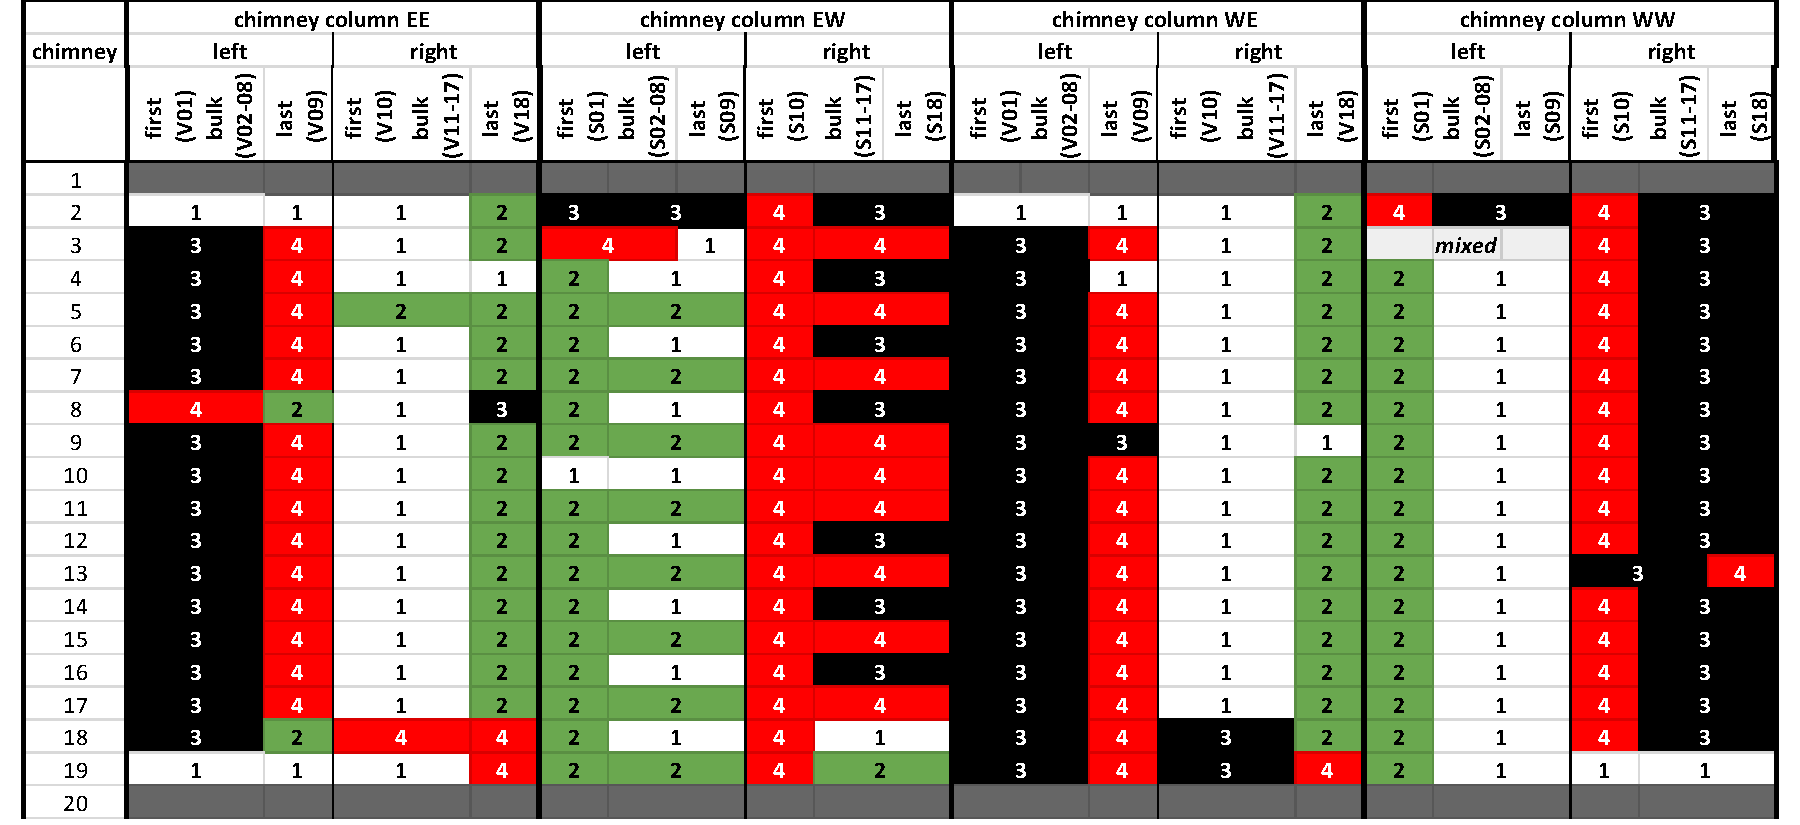
\includegraphics[width=16cm,angle=270]{fig/FinalTestPulseMap}\\
  }
  \caption{\label{fig:PulseCableMap}
    Pulse cable color (and number: see \cref{fig:FlangeConnections})
    used to test each cable.\\
    Each flange has six entries in the table, three for the left side and
    three for the right one.
    The first entry shows the pulse cable used to pulse the first 68-wire cable
    (V1 or S1), the second entry for the second to the eighth (V2--V8 or
    S2--S8), the third for last one (V9 or S9). The next three entries pertain
    cables V10 or S10, then V11--V17 or S11--S17, and finally V18 or S18.
  }
\end{figure}



\subsection{Collected data}
\label{ssec:data}

Data was collected systematically, in December 2018 for all chimneys except
for the four chimneys that were not yet installed: \Chimney{WE02},
\Chimney{WE03}, \Chimney{WE04} and \Chimney{WW02}. Further acquisition happened
on February 2019.
\\
After data acquisition, some flanges were replaced together with their \DBB's
That is the case for \Chimney{EE08}, \Chimney{WE02} and \Chimney{WW02}, the data
of which does not reflect the installed flanges any more.
In addition, \Chimney{WE03} and \Chimney{WE05} had one \DBB replaced after data
acquisition (DBB \#5 serving \Cable{V05} and \Cable{V14}, and DBB \#1 serving
\Cable{V01} and \Cable{V10}, respectively).
\\
The data is currently stored in ICARUS data area at \\
\texttt{/icarus/data/commissioning/connectivityTest/201812/chimney} \\
and archived in ICARUS dCache area at \\
\texttt{/pnfs/icarus/persistent/commissioning/connectivityTest/201812/archive}.\\
The data obsoleted by the changes reported above is still kept in the \texttt{old} subdirectory.



